\documentclass[10pt]{article}

\usepackage{graphicx}
\usepackage{amsmath,amsfonts,amssymb}

% use different colors for links:
\usepackage{color}
\definecolor{darkgreen}{rgb}{0.1,0.5,0.1}
\definecolor{darkblue}{rgb}{0.2,0.2,1.0}
\usepackage[colorlinks=true,linkcolor=darkblue,citecolor=darkblue,
            filecolor=darkblue,urlcolor=darkgreen]{hyperref}


\setlength{\textwidth}{6.2in}
\setlength{\oddsidemargin}{0.3in}
\setlength{\evensidemargin}{0in}
\setlength{\textheight}{8.9in}
\setlength{\voffset}{-1in}
\setlength{\headsep}{26pt}
\setlength{\parindent}{0pt}
\setlength{\parskip}{5pt}



% a few handy macros

\newcommand\matlab{{\sc matlab}}
\newcommand{\goto}{\rightarrow}
\newcommand{\bigo}{{\mathcal O}}
\newcommand{\half}{\frac{1}{2}}
%\newcommand\implies{\quad\Longrightarrow\quad}
\newcommand\reals{{{\rm l} \kern -.15em {\rm R} }}
\newcommand\complex{{\raisebox{.043ex}{\rule{0.07em}{1.56ex}} \hskip -.35em {\rm C}}}


% macros for matrices/vectors:

% matrix environment for vectors or matrices where elements are centered
\newenvironment{mat}{\left[\begin{array}{ccccccccccccccc}}{\end{array}\right]}
\newcommand\bcm{\begin{mat}}
\newcommand\ecm{\end{mat}}

% matrix environment for vectors or matrices where elements are right justifvied
\newenvironment{rmat}{\left[\begin{array}{rrrrrrrrrrrrr}}{\end{array}\right]}
\newcommand\brm{\begin{rmat}}
\newcommand\erm{\end{rmat}}

% for left brace and a set of choices
\newenvironment{choices}{\left\{ \begin{array}{ll}}{\end{array}\right.}
\newcommand\when{&\text{if~}}
\newcommand\otherwise{&\text{otherwise}}
% sample usage:
%  \delta_{ij} = \begin{choices} 1 \when i=j, \\ 0 \otherwise \end{choices}


% for labeling and referencing equations:
\newcommand{\eql}{\begin{equation}\label}
\newcommand{\eqn}[1]{(\ref{#1})}
% can then do
%  \eql{eqnlabel}
%  ...
%  \end{equation}
% and refer to it as equation \eqn{eqnlabel}.  


% some useful macros for finite difference methods:
\newcommand\unp{U^{n+1}}
\newcommand\unm{U^{n-1}}

% for chemical reactions:
\newcommand{\react}[1]{\stackrel{K_{#1}}{\rightarrow}}
\newcommand{\reactb}[2]{\stackrel{K_{#1}}{~\stackrel{\rightleftharpoons}
   {\scriptstyle K_{#2}}}~}

% Parts:

% set enumerate to give parts a, b, c, ...  rather than numbers 1, 2, 3...
\renewcommand{\theenumi}{\alph{enumi}}
\renewcommand{\labelenumi}{(\theenumi)}

% set second level enumerate to give parts i, ii, iii, iv, etc.
\renewcommand{\theenumii}{\roman{enumii}}
\renewcommand{\labelenumii}{(\theenumii)}

  % input some useful macros

\newcommand{\bv}{\bar v}


\begin{document}

% header:
\hfill\vbox{\hbox{AMath 586 / ATM 581}
\hbox{Homework \#5}\hbox{Due Thursday, June 13, 2019}}

{\bf Name:} Your name here
\vskip 5pt

Due to Canvas by 11:00pm PDT on the due date.

To submit, see \url{https://canvas.uw.edu/courses/1271892/assignments/4833214}



\noindent
\begin{itemize}
\item This final project is worth 65 points (same weight as the midterm).
\item Some additional extra credit problems will be available soon.
\item The description is long and has many parts, but much of the code
you'll need is similar to things you have already written or that is
provided in class notebooks.
\item Please submit Python codes or notebooks for all the problems.
\item Please write up your results nicely, preferably typeset and/or in Jupyter
notebooks, but this is not required.  
Ideally you might turn in a single notebook that works through all the
problems with appropriate discussion added in between. 
However you write it up, please 
organize things well and provide some discussion. 
\end{itemize} 

\vskip 10pt
\hrule
\vskip 10pt


First consider the ODE
\eql{ACode}
v'(t) = \frac 1 \epsilon g(v)
\end{equation}
where 
\eql{g}
g(v) = v(\alpha-v)(v-1)
\end{equation}
with $0<\alpha<1$.

This equation has three possible steady
state solutions: $v(t)\equiv 0$, $v(t)\equiv \alpha$, $v(t)\equiv 1$.
The middle one
is an {\it unstable} steady state.  If $v(0) = \alpha + \delta$ with
$\delta$ small but nonzero, then $v(t)$ moves away from $\alpha$, towards 0
if $\delta<0$ or towards 1 if $\delta>0$.  These are the two stable steady
states.  The parameter $\epsilon>0$ controls the rate of decay towards these
steady states.  For small $\epsilon$ the solution moves rapidly towards 0 or
1.

%--------------------------------------------------------------------------
\vskip 10pt
\hrule
\vskip 10pt
{\large\bf Problem 1.} \vskip 5pt
Set $\alpha = 0.3$ and $\epsilon = 1$.
Use {\tt scipy.integrate.odeint} (or {\tt scipy.integrate.solve\_ivp}
if you prefer) in Python to plot solutions curves $v(t)$ for several
different initial values $v(0)$ lying between 0 and 1, in particular
for {\tt v0 = linspace(0,1,11)}.  Plot all these curves $v(t)$ for
$0\leq t \leq 10$ on a single plot.

Produce similar plots for $\epsilon = 0.1$ and $\epsilon = 0.05$.

%--------------------------------------------------------------------------
\vskip 10pt
\hrule
\vskip 10pt
{\large\bf Problem 2.} \vskip 5pt

(a) Implement the Forward Euler method to solve this problem.  Since it is a
scalar nonlinear problem, the Jacobian is simply the derivative of the right-hand
side in \eqn{ACode}.  Based on this function and assuming $v$ stays between 
0 and 1, estimate the stability limit for Forward Euler as a function of 
$\epsilon$ for $\alpha = 0.3$.  Experiment with different values of $\epsilon$ 
and different time steps to see if this gives reasonable guidance and 
provide some plots and discussion.  Is it reasonable to assume $v$ stays within
these bounds?

(b) Do the same for the 2-stage explicit Runge-Kutta method given by (5.30) in 
the book.  Explain any curious behavior, in particular with $\epsilon=0.01$,
$\eta = 0.6$, and 22 time steps (up to $t=1$) you should obtain something
like this figure:

\hfil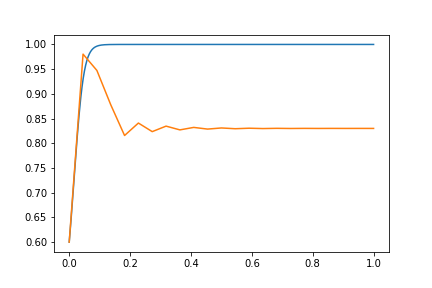
\includegraphics[width=3.5in]{figs/RK2ex1.png}\hfil

Why does it seem to tend to a non-physical steady state with this method?
Can you determine the value it tends to from the ODE and method?

(c) Implement the Backward Euler method for this problem and confirm that it 
remains stable and behaves well for much larger time steps that what would
be allowed by the explicit methods.
\vskip 10pt
\hrule
\vskip 10pt
%--------------------------------------------------------------------------

{\bf The Allen-Cahn Equation.}
We can turn \eqn{ACode} into a PDE in one
space dimension and time by letting $v(x,t)$ vary in space and adding
spatial diffusion, obtaining
\eql{AC1d}
v_t(x,t) = \kappa v_{xx}(x,t) + \frac 1 \epsilon g(v).
\end{equation}
This is a scalar reaction-diffusion equation, a variant of the {\it
Allen-Cahn equation} that is used as a simple model of phase transition.

The lower stable steady state at $v=0$
corresponds to a material in one phase (e.g.
solid) while the upper stable steady state  at $v=1$
corresponds to a different phase
(e.g. liquid).  

Consider initial data
\eql{ACv0}
v(x,0) = \begin{choices} 1 \when x<0 \\  0 \when x\geq 0 \end{choices}
\end{equation}
and the Cauchy problem on $-\infty<x<\infty$ so we don't have to worry about
boundary conditions for the moment.

If $\kappa = 0$ (no diffusion) then $v(x,t) = v(x,0)$ for all time since
both $v=1$ and $v=0$ are steady states and so $v_t\equiv 0$.  With diffusion,
however, this step discontinuity immediately smooths out and $v(x,t)$ for
$t>0$ will be a continuous function taking all values between 0 and 1.  For
these values of $v$ the reaction term drives $v$ back towards 0 (where
$v<\alpha$) or towards 1 (where $v>\alpha$), tending to sharpen the smeared
profile back towards a step discontinuity.  There is a competition between
the smearing effect of diffusion and the sharpening effect of the reaction,
leading to a steady profile that is smeared to a finite degree that depends
on the relation between the parameters $\epsilon$ and $\kappa$.

The smearing effect of diffusion is symmetric about $v=1/2$: for
$\epsilon\goto\infty$ the solution to the pure diffusion equation with data
\eqn{ACv0} has $v>1/2$ for $x<0$ and $v<1/2$ for $x>0$ and appears symmetric
about this point.
The sharpening from the reaction term is also symmetric about $v=1/2$ if
$\alpha = 1/2$.  In this case $v(x,t)$ approaches a steady state profile
$v(x,t) \goto \bv(x/\delta)$ as $t\goto \infty$.
A new parameter $\delta$ has been introduced that will be related to
$\kappa$ and $\epsilon$ below.  The idea is that the profile $\bv(\xi)$
should be independent of the parameters $\kappa$ and $\epsilon$ but is
rescaled based on these parameters since the width of the transition from
$v=1$ to $v=0$ will depend on these parameters.

We can determine $\delta$ and $\bv$ by inserting $v(x,t) = \bar
v(x/\delta)$ into the PDE \eqn{AC1d}, obtaining a
boundary value problem
\eql{ACbvp}
0= \frac{\kappa}{\delta^2} \bv''(x/\delta) + \frac 1 \epsilon g(\bar
v(x/\delta)).
\end{equation}
Multiplying by $\delta^2 / \kappa$ and rearranging gives
\eql{ACbvp2}
\bv''(x/\delta) = -  \frac {\delta^2}{\kappa\epsilon} g(\bar
v(x/\delta)).
\end{equation}
This suggests that we should choose $\delta^2$ to be proportional to
$\kappa\epsilon$ in order to obtain an ODE for $\bv$ that is independent
of the parameters.  In order to easily solve the resulting BVP it is
convenient to choose
\eql{delta}
\delta = \sqrt{2\kappa\epsilon}.
\end{equation}
Setting $\xi = x/\delta$ then gives the ODE for $\bv(\xi)$,
\eql{ACbvp3}
\bv''(\xi) = -2\bv(\xi)(1/2 - \bv(\xi))(\bv(\xi)-1).
\end{equation} 
with asymptotic boundary conditions $\bv(x)\goto 1$ as $x\goto -\infty$
and $\bv(x)\goto 0$ as $x\goto \infty$.  We also want $\bv(\xi)$ to be
centered about $\xi=0$, so we would like $v(0) = 1/2$.

Note that even without solving the ODE \eqn{ACbvp3} we can deduce that the
width of the transition zone in the traveling wave is proportional to
$\delta$ and hence to $\sqrt{\kappa\epsilon}$.  This information might be
useful if we wanted to use a nonuniform grid to solve the problem
numerically, or to choose an appropriate value of $h$ for a uniform grid.

\vskip 10pt
\hrule
\vskip 10pt
%--------------------------------------------------------------------------

{\large\bf Problem 3.} \vskip 5pt
Show that the function 
\eql{bv}
\bv(\xi) = \frac{1}{1 + \exp(\xi)}
\end{equation}
satisfies both of the equations
\eql{bv1}
\bv'(\xi) = -\bv(\xi)(1-\bv(\xi))
\end{equation}
and
\eql{bv2}
\bv''(\xi) = 2\bv(\xi)(1-\bv(\xi))(1/2 - \bv(\xi)),
\end{equation}
and also satisfies 
\eql{bvbc}
\begin{split}
&\bv(\xi) \goto 1 \quad\mbox{as}\quad \xi\goto -\infty,\\
&\bv(\xi) \goto 0 \quad\mbox{as}\quad \xi\goto +\infty,\\
&\bv(0) = 1/2.
\end{split}
\end{equation}
Hence this is a steady state solution for the case $\alpha = 1/2$.

\vskip 10pt
\hrule
\vskip 10pt
%--------------------------------------------------------------------------


If $\alpha \neq 1/2$ then the effect of the reaction term is not symmetric.
If $0<\alpha<1/2$ then some values of $v$ less than 1/2 are driven towards
$v=1$ by the reaction term.  When coupled with the symmetric diffusion this
leads to a traveling wave propagating with some velocity $c$ that is
positive if $\alpha<1/2$ or negative if $\alpha>1/2$.  
The traveling wave profile is given by the same function $\bv(x)$ that
satisfies the boundary value problem \eqn{ACbvp3}, and that the traveling
wave has the form
\eql{ACtrav}
v(x,t) = \bv((x-ct)/\delta),
\end{equation}
where the speed $c$ is given by
\eql{speed}
c = \sqrt{\frac{2\kappa}{\epsilon}} \left(\half - \alpha\right).
\end{equation}

\newpage

\vskip 10pt
\hrule
\vskip 10pt
%--------------------------------------------------------------------------
{\large\bf Problem 4.} \vskip 5pt
\begin{enumerate}
\item For any $0<\alpha<1$, show that $v(x,t) = \bv((x-ct)/\delta)$ is a
traveling wave solution to \eqn{AC1d} provided that $c$ satisfies
\eqn{speed}.

\item Suppose we define the width of the transition zone (wave front)
in a traveling wave
to be the distance in $x$ over which $v$ falls from 0.99 to 0.01.  Show that
the width of wave front is roughly $9\delta$.  This can be used to choose a
suitable value of $h$.  For example, choosing $h\approx \delta$ would give
roughly 9 grid points in the wave front, which is probably about the minimum
needed to resolve it well numerically.
\end{enumerate} 

\vskip 10pt
\hrule
\vskip 10pt
%--------------------------------------------------------------------------

{\large\bf Problem 5.} \vskip 5pt

(a) Implement a {\em fractional step method} to approximate solutions to the
Allen-Cahn equation on the interval $-1 \leq x \leq 3$ with initial data
$v(x,0) = V(x/\delta)$, where $\delta$ is determined from specified values
of $\kappa = 0.3$ and $\epsilon$.  

Each time step, first take a time step of the diffusion equation, and then a
time step of the nonlinear ODEs (at each grid point).

Your code should use: 
\begin{itemize} 
\item The Crank-Nicolson method for the diffusion equation. 
You might want to use code from the notebook {\tt notebooks/HeatEquation.ipynb}
for the diffusion part.  Adapt this to work on the interval $-1 \leq x \leq 3$.
\item To solve the ODE in each timestep, use either
the Forward Euler method, the two-stage explicit Runge-Kutta method (5.30), 
or the Backward Euler method.  Introduce a parameter {\tt odemethod}
in the input data of your function to select one of these.
Note that for Backward Euler, an implicit nonlinear equation must be solved at 
each grid point (in every time step).  You can use {\tt scipy.optimize.fsolve}
for these.
\item Similar to {\tt notebooks/HeatEquation.ipynb}, set initial condition and
boundary conditions in each time step using 
a function {\tt utrue} that implements the true solution for a traveling wave.
\end{itemize} 

(b) Test your method using $\alpha=0.3$ and $\epsilon = 0.01$ with
initial data given by the exact traveling wave solution at $t=0$,
going up to time $t=1$, and plotting both the exact and computed
solution for comparison.  Produce some plots of the solution to
show that the code works with both ODE solvers.

You should see results like this for the case when Forward Euler is used and
$m=49$ with 100 time steps up to time 1:

\hfil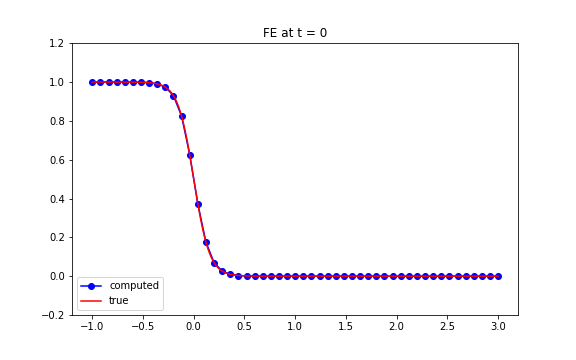
\includegraphics[width=2.8in]{figs/ACwithFE0.png}\hfil
\hfil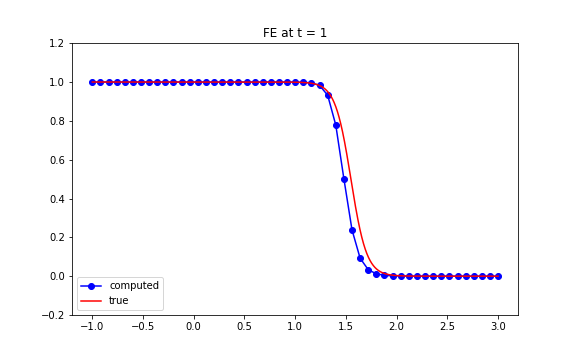
\includegraphics[width=2.8in]{figs/ACwithFE1.png}\hfil


(c) What order of accuracy do you observe for each choice of ODE solver?
Test by refining in space and time with $k/h$ fixed (for $\alpha=0.3$ and
$\epsilon = 0.01$) and produce a log-log plot of the errors in each case.

(d) Test your code also with $\alpha = 0.5$ and $\alpha = 0.7$ and verify
that it gives the expected solutions in these cases.  (You don't need to
repeat the convergence test for these values.)

%--------------------------------------------------------------------------


\vskip 10pt
\hrule
\vskip 10pt
%--------------------------------------------------------------------------
{\large\bf Problem 6.} \vskip 5pt

Now try using $\epsilon = 0.003$ with $\alpha=0.3$ 
and a grid with $m=49$ and 45 time steps over up to a final time of 0.5 
(a shorter time interval since with smaller $\epsilon$ the wave 
propagates faster).

When using Backward Euler for the ODE term, you should see results like shown 
in this figure:

\hfil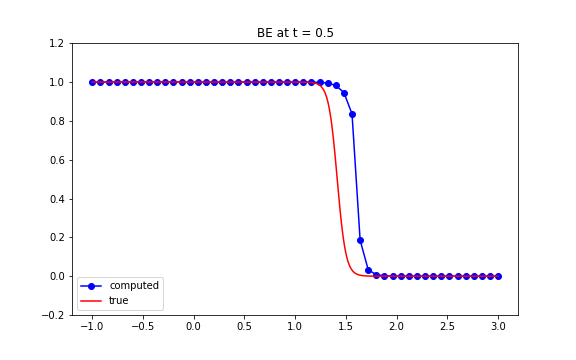
\includegraphics[width=3.5in]{figs/ACwithBE.png}\hfil

The wave appears stable, but moves at the wrong speed. This could be quite
misleading if we didn't know the true solution! 

For these values of $\epsilon$ and $\alpha$, experiment with different 
resolutions in space and in time to explore how the numerical solution behaves,
both when the Forward Euler method and when the Backward Euler method 
are used.  Given that the implicit ODE method requires a lot more work than the
explicit method (solving a nonlinear equation at every grid point, every time
step), try to reach some conclusions on whether it is worthwhile to use
the implicit ODE solver for this Allen-Cahn problem.  (Recall that Problems
2(a) and 4(b) give some ideas on what sort of resolution might be needed
in time and space).

This problem is a bit open-ended.  Feel free to experiment with other values
of $\epsilon$ too if useful (or other variations). A variety of different
wrong numerical solutions can be generated depending on parameter choices.

\end{document}
